\documentclass[a4paper]{article}
% Leave uncommented if the LaTeX file is uploaded to arXiv.org
\pdfoutput=1
\pdfminorversion=7

% Packages
\usepackage{arxiv}
\usepackage[colorlinks=true,linkcolor=cyan,citecolor=cyan]{hyperref}
\usepackage[numbers]{natbib}
\usepackage{authblk}
\usepackage{caption}
\usepackage{subcaption}
\usepackage{graphicx}
\usepackage{amsmath}
\usepackage{amssymb}
\usepackage{epstopdf}
\usepackage{comment}
\usepackage{xcolor}
\usepackage{float}
\usepackage{doi}

% Useful macros for equations and units in HEP
\newcommand*{\TeV}{\text{ TeV}}
\newcommand*{\GeV}{\text{ GeV}}
\newcommand*{\MeV}{\text{ MeV}}
\newcommand*{\keV}{\text{ keV}}
\newcommand*{\eV}{\text{ eV}}
\newcommand*{\meV}{\text{ meV}}
\newcommand*{\bb}{\boldsymbol}
\newcommand*{\beqn}{\begin{equation}}
\newcommand*{\eeqn}{\end{equation}}
\newcommand{\req}[1]{Eq.\,(\ref{#1})}
\newcommand{\rf}[1]{Fig.~{\ref{#1}}}
\newcommand{\rsec}[1]{Sect.\,{\ref{#1}}}

% Useful macros for annotation
\newcommand*{\xred}{\color{red}}
\newcommand*{\xblue}{\color{black}}
\newcommand*{\xgreen}{\color{green}}

%\title{\boldmath Magnetic Properties of Finite Temperature Primordial Electron-Positron Plasma}
\title{\boldmath Spin paramagnetic origins of cosmic magnetism:\\ A first look}
% Future paper title: Primordial Universe Ferromagnetism

% Author Orcid ID: Define per author
\newcommand{\orcA}{0000-0001-8217-1484}
\newcommand{\orcB}{0000-0001-5038-8427}
\newcommand{\orcC}{0000-0001-5474-2649}

\author{Andrew Steinmetz\orc{\orcC}%\thanks{Correspondence: \texttt{ajsteinmetz@arizona.edu}}
, Cheng Tao Yang\orc{\orcB}, and Johann Rafelski\orc{\orcA}\\ Department of Physics, The University of Arizona, Tucson, AZ 85721, USA}

\begin{document}

\maketitle

\begin{abstract}
    We explore the hypothesis that spin polarization in the primordial electron-positron $(e^{+}e^{-})$ plasma in the temperature range $2,000\keV>T>20\keV$ is responsible for the magnetic fields we see in the universe today. We characterize the paramagnetic nature of the $e^{+}e^{-}$ plasma and determine that only a small polarization asymmetry is required to produce self-magnetization consistent with contemporary field strengths.
\end{abstract}

\keywords{early universe cosmology \and magnetization \and electron-positron plasma \and intergalactic magnetic fields}

%%%%%%%%%%%%%%%%%%%%%%%%%%%%%%%%%%%%%%%
\section{Introduction}
\label{sec:introduction}
\noindent  
Considering the ubiquity of magnetic fields~\cite{giovannini2003magnetized,kronberg1994extragalactic} in the universe, we search for a primordial mechanism which could produce {\xblue the diversity of magnetism observed today.} Macroscopic domains of magnetic fields have been found around compact objects (stars, planets, etc.); between stars; within galaxies; between galaxies in clusters; and surprisingly in deep extra-galactic void spaces. The conventional elaboration of the origins for cosmic  primordial magnetic fields (PMF) are detailed in~\cite{gaensler2004origin,durrer2013cosmological,batista2021gammaray}.

Intergalactic magnetic field (IGMF) are  difficult to measure and difficult to explain. {\xblue In this work, IGFM will refer to experimentally observed intergalactic fields of any origin while PMF refers to fields generated via primordial (early universe) processes.} The bounds for IGMF at a length scale of $1{\rm\ Mpc}$ are today~\cite{neronov2010evidence,taylor2011extragalactic,pshirkov2015new,jedamzik2019stringent,vernstrom2021discovery}
\begin{align}
    \label{igmf}
    10^{-8}{\rm\ G}>\mathcal{B}_{\rm IGFM}>10^{-16}{\rm\ G}\,.
\end{align}
Faraday rotation from distant radio active galaxy nuclei (AGN)~\cite{pomakov2022redshift} suggest that neither dynamo nor astrophysical processes would sufficiently account for the presence of magnetic fields in the universe today if the IGMF strength was around the upper bound of ${\cal B}_{\rm IGMF}\simeq30-60{\rm\ nG}$ as found in Ref.~\cite{vernstrom2021discovery}. Such strong magnetic fields would then require that at least some portion of the IGMF arise from primordial sources that predate the formation of stars.

We investigate the hypothesis that the observed  IGMF  are primordial in nature, predating even the recombination epoch. Specifically, we explore the role of the relatively large electron-positron $(e^{+}e^{-})$ pair abundance which only disappears well after Big Bang nucleosynthesis (BBN). {\xblue Electrons and positrons, having the largest magnetic moments in nature, are likely to have been magnetized in the pre-BBN early universe due to spin orientation. The rapid $10^{8}$ drop in $e^{+}e^{-}$ abundance within the narrow temperature range $200\keV>T>20\keV$ shown in \rf{fig:densityratio} should then be capable of inducing dynamical currents preserving magnetic flux} in the emerging $p,\alpha,e^-$ plasma.  
%%%%%%%%%%%%%%%%%%%%%%%%%%%%%%%%%%%%%%%
\begin{figure}[ht]
    \centering
    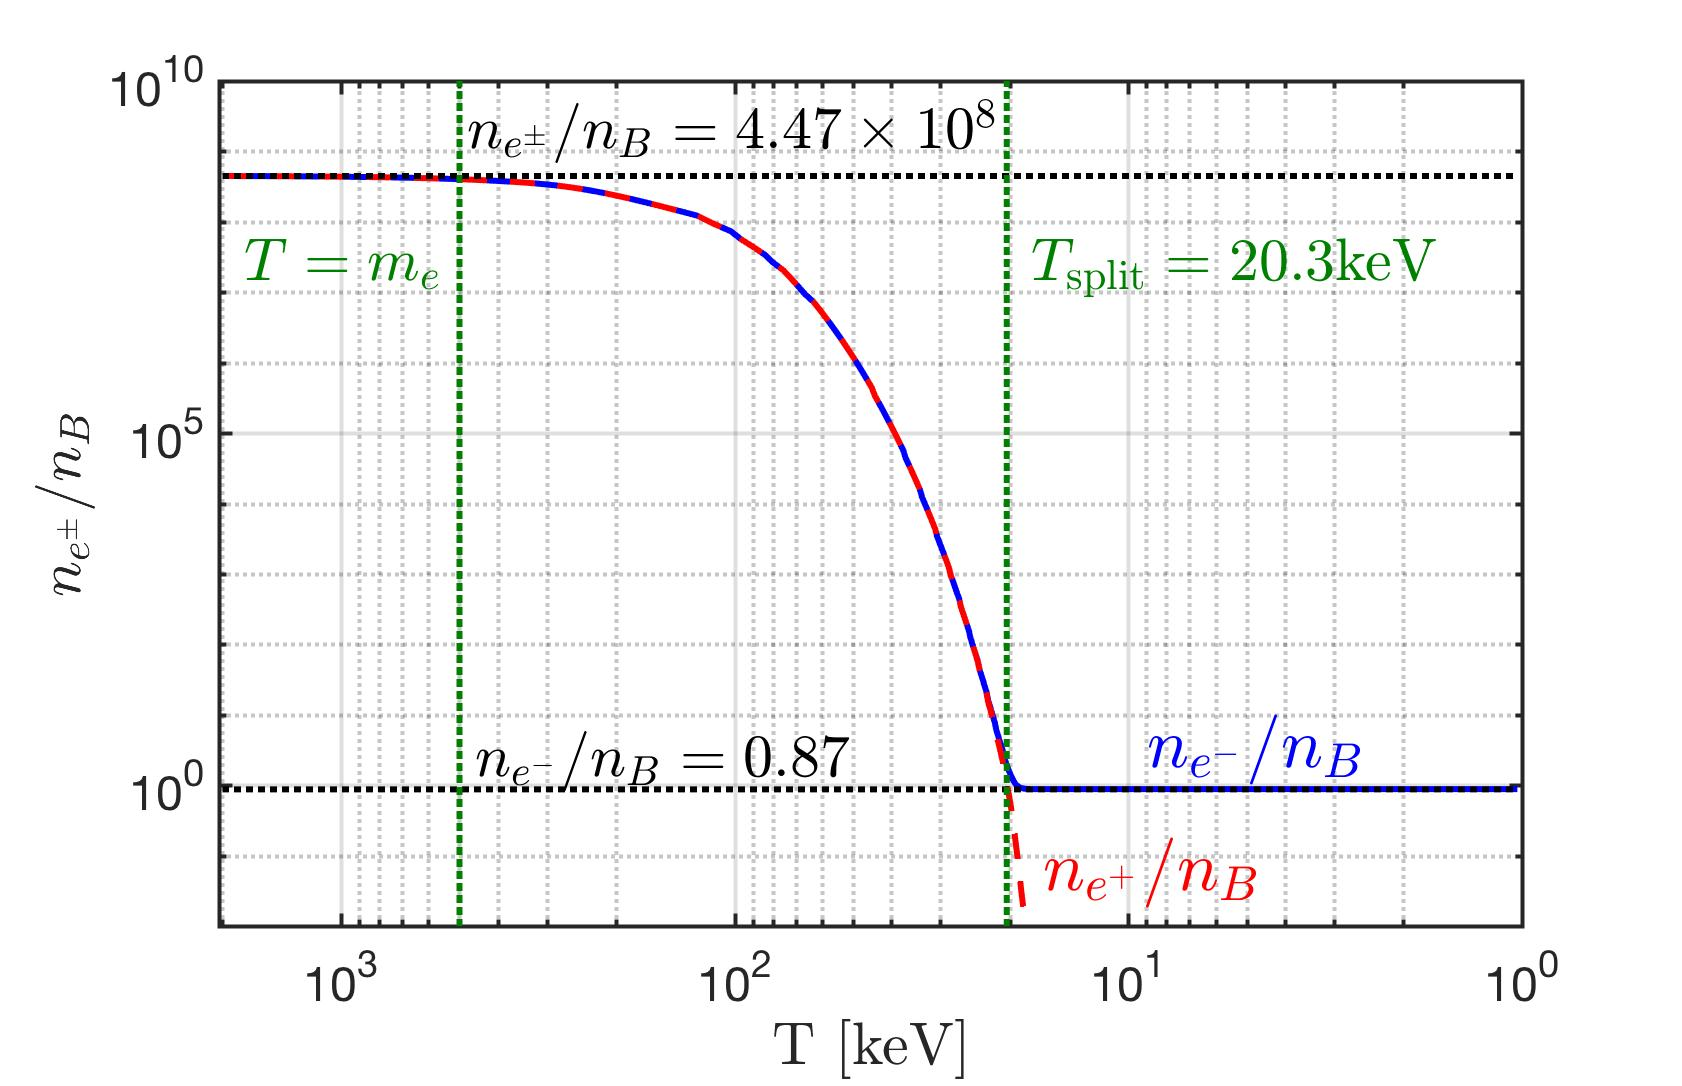
\includegraphics[width=0.8\textwidth]{plots/EEPlasmaDensityRatio_new.jpg}
    \caption{Electron $e^-$ and positron $e^+$ to baryon ratio $n_{e^{\pm}}/n_{B}$  as a function of photon temperature in the universe. See text for further details.}
    \label{fig:densityratio} 
\end{figure}
%%%%%%%%%%%%%%%%%%%%%%%%%%%%%%%%%%%%%%%

Large pre-recombination primordial fields could therefore lead to early universe baryon inhomogeneities which in turn would produce anisotropies in the cosmic microwave background (CMB)~\cite{jedamzik2013smallscale,abdalla2022cosmology}. Jedamzik and Pogosian~\cite{jedamzik2020relieving} propose further that the presence of ${\cal B}_{\rm PMF}\simeq0.1{\rm\ nG}$ could be sufficient to explain the Hubble tension. {\xblue We consider an entirely novel hypothesis that the primordial magnetization of the universe is driven by spin paramagnetism originating in the relatively dense electron-positron $e^{+}e^{-}$ plasma which reached about 100 million pairs per baryon at the pre-BBN temperature $T=200\keV$ (see: \rf{fig:densityratio}). These results were obtained using charge neutrality and the baryon to photon content (entropy) of the universe~\cite{rafelski2023short}.} 

{\xblue The electron-to-baryon ratio $n_{e^{-}}/n_{B}$ is shown in \rf{fig:densityratio} as the solid blue line which overlaps the positron-to-baryon ratio $n_{e^{+}}/n_{B}$, represented by the dashed red line, until the temperature drops below $T_{\rm split}=20.3\keV$ as the abundances of the two species diverge from one another.} The two vertical dashed green lines denote temperatures $T=m_{e}\simeq511\keV$ and $T_{\rm split}=20.3\keV$. {\xblue It is customary to show time as increasing from left to right which corresponds to a decreasing temperature. All figures in this paper will plot temperature as the $x$-axis scale.} The two horizontal black dashed lines denote the relativistic $T\gg m_e$ abundance of $n_{e^{\pm}}/n_{B}=4.47\times10^{8}$ and post-annihilation {\xblue abundance of  $n_{e^{-}}/n_{B}=0.87$. The deviation from unity in the post-annihilation abundance reflects the presence of bound neutrons in the baryon content.} Above temperature $T\simeq85\keV$, the $e^{+}e^{-}$ primordial plasma density exceeded that of the Sun's core density $n_{e}\simeq6\times10^{26}{\rm\ cm}^{-3}$~\cite{bahcall2001solar}. 

{\xblue Our analysis of the relativistic fermion partition function focuses} on the spin contribution to magnetization. {\xblue At $T\simeq200\keV$, due to very high $e^{+}e^{-}$ pair densities, we believe that spin paramagnetism is dominant over Landau orbital diamagnetism.} We show that magnetization is nonzero {\xblue even for a nearly symmetric particle-antiparticle gas as well as account for the matter-antimatter asymmetry present in the universe.} We further demonstrate that magnetization can spontaneously increase in strength near the IGMF upper limit seen in \req{igmf}. This is assisted by the fact that antiparticles $(e^{+})$ have the opposite sign of charge, and thus magnetic moment, compared to particles  $(e^{-})$. {\xblue Therefore in an $e^{+}e^{-}$ pair plasma, net magnetization can be associated with opposite spin orientations for particles and antiparticles without the accompaniment of} a net angular momentum in the volume considered. This is of course very different from the the matter dominated universe arising below $T\simeq20\keV$ which includes the current epoch.

%%%%%%%%%%%%%%%%%%%%%%%%%%%%%%%%%%%%%%%
\section{Electron-positron abundance}
\label{sec:abundance}
%%%%%%%%%%%%%%%%%%%%%%%%%%%%%%%%%%%%%%%
\noindent As the universe cooled below temperature $T=m_{e}$ (the electron mass), the thermal electron and positron comoving density {\xblue of $n_{e^{\pm}}/n_{B}=4.47\times10^{8}$} depleted falling over eight orders of magnitude. At $T_{\rm split}=20.3\keV$, the charged lepton asymmetry (mirrored by baryon asymmetry {\xblue and enforced by charge neutrality}) became evident {\xblue as the surviving excess electrons persisted while positrons vanished entirely from the particle inventory of the universe. Conversion of the dense $e^{+}e^{-}$ pair plasma into photons reheated the photon background~\cite{birrell2014relic} separating the photon and neutrino temperatures. The $e^{+}e^{-}$ annihilation and photon reheating period lasted no longer than an afternoon lunch break.} Because of charge neutrality, the post-annihilation comoving ratio $n_{e^{-}}/n_{B}=0.87$~\cite{rafelski2023short} is slightly offset from unity in~\rf{fig:densityratio} by the presence of bound neutrons in $\alpha$ particles and  other neutron containing light elements produced during BBN epoch. 

{\xblue To obtain a quantitative description of the above evolution, we study the bulk properties of the relativistic charged/magnetic gasses in a nearly homogeneous and isotropic primordial universe via} the thermal Fermi-Dirac or Bose distributions. {\xblue For matter $(\sigma=+1)$ and antimatter $(\sigma=-1)$ particles, a nonzero chemical potential $\mu_{\sigma}=\sigma\mu$ is caused by an imbalance of matter and antimatter. While the primordial electron-positron plasma era was overall charge neutral, there was a small asymmetry in the charged leptons from baryon asymmetry~\cite{fromerth2012quarkgluon,canetti2012matter} in the universe. Consideration of reactions such as $e^+e^-\leftrightarrow\gamma\gamma$ constrains the chemical potentials of electrons and positrons~\cite{elze1980relativistic} as 
\begin{align}
    \label{cpotential}
    \mu\equiv\mu_{e^{-}}=-\mu_{e^{+}}\,,\qquad
    \lambda\equiv\lambda_{e^{-}}=\lambda_{e^{+}}^{-1}=\exp\frac{\mu}{T}\,,
\end{align}
where $\lambda$ is the fugacity of the system.} 

{\xblue During the $e^{+}e^{-}$ plasma epoch, the density changed dramatically over time (see: \rf{fig:densityratio}) changing the chemical potential in turn. We can then parameterize the chemical potential of the $e^{+}e^{-}$ plasma as a function of temperature $\mu\rightarrow\mu(T)$ via the charge neutrality of the universe which implies}
\begin{align}
    \label{chargeneutrality}
    n_{p}=n_{e^{-}}-n_{e^{+}}=\frac{1}{V}\lambda\frac{\partial}{\partial\lambda}\ln{\cal Z}_{e^{+}e^{-}}\,.
\end{align}
{\xblue In \req{chargeneutrality}, $n_{p}$ is the observed total number density of protons in all baryon species. The parameter $V$ relays the proper volume under consideration and $\ln{\cal Z}_{e^{+}e^{-}}$ is the partition function for the electron-positron gas. The chemical potential defined in \req{cpotential} is obtained from the requirement that the positive charge of baryons (protons, $\alpha$ particles, light nuclei produced after BBN) is exactly and locally compensated by a tiny net excess of electrons over positrons.}

{\xblue The abundance of baryons is itself fixed by the known abundance relative to photons~\cite{workman2022pdg} and we employed the contemporary recommended value $n_B/n_\gamma=6.09\times 10^{-10}$.} The resulting chemical potential  needs to be evaluated carefully to obtain the behavior near to $T_{\rm split}=20.3\keV$ where the relatively {\xblue small value of chemical potential $\mu$} rises rises rapidly so that positrons vanish from the particle inventory of the universe while nearly one electron per baryon remains. The detailed solution of this problem is found in Refs.\;\cite{fromerth2012quarkgluon,rafelski2023short} leading to the results shown in \rf{fig:densityratio}. These results are obtained allowing for Fermi-Dirac and Bose statistics, however it is often numerically sufficient to consider the Boltzmann distribution limit.

In the presence of a magnetic field ${\cal B}$ there is some modification of the usual relativistic fermion partition function which is now given  by
\begin{align}
    \label{partition}
    \ln{\cal Z}_{e^{+}e^{-}}=\frac{e{\cal B}V}{(2\pi)^{2}}\sum_{\sigma}^{\pm}\sum_{s}^{\pm}\sum_{n=0}^{\infty}\int_{-\infty}^{\infty}{\rm d}p_{z}\left[\ln\left(1+\lambda_{\sigma}\xi_{s}e^{-E_{n}^{s}/T}\right)\right]\,,\qquad\Upsilon_{\sigma}^{s}=\lambda_{\sigma}\xi_{s}=\exp{\frac{\mu_{\sigma}+\eta_{s}}{T}}\,,
\end{align}
{\xblue with electric charge $e\equiv q_{e^{+}}=-q_{e^{-}}$.} The index $\sigma$ in \req{partition} is a sum over electron and positron states while $s$ is a sum over polarizations. Since we are interested in small asymmetries (e.g. baryon excess over antibaryons, one spin polarization over another) we introduce the generalized particle fugacity $\Upsilon_{\sigma}^{s}$ as the product of:
\begin{itemize}
    \item[a.] Chemical fugacity $\lambda_{\sigma}$
    \item[b.] Spin fugacity $\xi_{s}$
\end{itemize}
The chemical fugacity $\lambda_{\sigma}$ {\xblue (defined in \req{cpotential} above) describes deformation of the Fermi-Dirac distribution due to nonzero chemical potential $\mu$.} An imbalance in electrons and positrons leads {\xblue as discussed earlier} to a nonzero particle chemical potential $\mu\neq0$. We then introduce a novel spin fugacity $\xi_{s}$ and spin potential $\eta_{s}=s\eta$. {\xblue We propose the spin potential follows analogous expressions as seen in \req{cpotential} obeying
\begin{align}
    \label{spotential}
    \eta\equiv\eta_{+}=-\eta_{-}\,,\qquad
    \xi\equiv\xi_{+}=\xi_{-}^{-1}= \exp{\frac{\eta}{T}}\,.
\end{align}

An imbalance in spin polarization within a region of volume $V$ results in a nonzero spin potential $\eta\neq0$. Conveniently since antiparticles have opposite sign of charge and magnetic moment, the same magnetic moment is associated with opposite spin orientation for particles and antiparticles independent of degree of spin-magnetization. A completely particle-antiparticle symmetric magnetized plasma will have therefore zero total spin angular momentum and zero spin potential $\eta=0$. This is of course very different from the situation today of a matter dominated universe.}

%%%%%%%%%%%%%%%%%%%%%%%%%%%%%%%%%%%%%%%
\section{Primordial paramagnetism }
\label{sec:fugacity}
%%%%%%%%%%%%%%%%%%%%%%%%%%%%%%%%%%%%%%%
\noindent
As the universe undergoes isotropic expansion, the temperature decreases {\xblue adiabatically~\cite{abdalla2022cosmology} and conserving entropy} as 
\begin{align}
    \label{tscale}
    T(t)=T_{0}\frac{a_{0}}{a(t)}\rightarrow T(z)=T_{0}(1+z)\,,
\end{align}
where $a(t)$ is the scale factor defined by the FLRW metric~\cite{weinberg1972gravitation} and $z$ is the redshift. The comoving temperature $T_{0}$ is given by the present day temperature of the CMB, with contemporary scale factor $a_{0}=1$. Within a homogeneous magnetic domain, the magnetic field varies~\cite{durrer2013cosmological} over cosmic expansion as
\begin{align}
    \label{bscale}
    {\cal B}(t)={\cal B}_{0}\frac{a_{0}^{2}}{a^{2}(t)}\rightarrow{\cal B}(z)={\cal B}_{0}\left(1+z\right)^{2}\,,
\end{align}
where ${\cal B}_{0}$ is the comoving value of the magnetic field obtained from the contemporary value of the magnetic field today  given in \req{igmf}. Non-primordial magnetic fields (which are generated through other mechanisms  such as dynamo or astrophysical sources) do not follow this scaling~\cite{pomakov2022redshift}. The presence of matter and late universe structure formation also  contaminates the primordial field evolution in \req{bscale}. It is only in deep intergalactic space where primordial fields remain preserved and comoving over cosmic time.

From \req{tscale} and \req{bscale} emerges a natural ratio of interest here which is conserved over cosmic expansion 
\begin{align}
    \label{tbscale}
    b \equiv\frac{e{\cal B}(t)}{T^{2}(t)}=\frac{e{\cal B}_{0}}{T_{0}^{2}}\equiv b_0={\rm\ const.}\qquad10^{-3}>b_{0}>10^{-11}\,,
\end{align}
given in natural units ($c=\hbar=k_{B}=1$). We computed the bounds for this cosmic magnetic scale ratio by using the present day observations given by \req{igmf} and the present CMB temperature $T_{0}=2.7{\rm\ K}\simeq2.3\times10^{-4}\eV$~\cite{aghanim2018planck}.

To evaluate paramagnetic properties of the $e^-e^+$ pair plasma we take inspiration from Ch. 9 of Melrose's treatise on magnetized plasmas~\cite{melrose2008quantum}. We focus  on the bulk properties of thermalized plasmas in (near) equilibrium. In considering $e^{+}e^{-}$ pair plasma, we introduce the microscopic energy of the charged $\pm e$ relativistic fermion within a homogeneous ($z$-direction) magnetic field~\cite{steinmetz2018magnetic}. The energy eigenvalue is given by
\begin{align}
    \label{kgp}
    E^{\pm}_{n}(p_{z},{\cal B})=\sqrt{m_{e}^{2}+p_{z}^{2}+e{\cal B}\left(2n+1\mp\frac{g}{2}\right)}\,,\qquad n\in0,1,2,\ldots
\end{align}
where $p_{z}$ is the momentum parallel to the field axis and $n$ is the Landau orbital quantum number. The {\xblue superscript} $\pm$ refers to the spin polarization along the field axis: parallel $(s=+1)$ or anti-parallel $(s=-1)$ {\xblue for both particle and antiparticle species.} The parameter $g$ is the gyro-magnetic ($g$-factor) of the particle. As statistical properties depend on the characteristic Boltzmann factor $E/T$, another interpretation of \req{tbscale} in the context of energy eigenvalues (such as those given in \req{kgp}) is the preservation of magnetic moment energy relative to momentum under adiabatic cosmic expansion.

We rearrange \req{kgp} by pulling the spin dependency and the ground state Landau orbital into the mass writing
\begin{align}
    \label{effmass}
    E^{\pm}_{n}={\tilde m}_{\pm}\varepsilon_{n}^{\pm}(p_{z},{\cal B})={\tilde m}_{\pm}\sqrt{1+\frac{p_{z}^{2}}{{\tilde m}_{\pm}^{2}}+\frac{2e{\cal B}n}{{\tilde m}_{\pm}^{2}}}\,,\qquad {\tilde m}_{\pm}^{2}=m_{e}^{2}+q{\cal B}\left(1\mp\frac{g}{2}\right)\,,
\end{align}
where we introduced the {\xblue dimensionless energy $\varepsilon^{\pm}_{n}$ and} effective polarized mass ${\tilde m}_{\pm}$ which is distinct for each spin alignment and is a function of magnetic field strength ${\cal B}$. The effective polarized mass ${\tilde m}_{\pm}$ allows us to describe the $e^{+}e^{-}$ plasma with the spin effects almost wholly separated from the Landau characteristics of the gas when considering the plasma's thermodynamic properties.

Since {\xblue we address} the temperature interval where {\xblue the effects of quantum Fermi statistics on the $e^{+}e^{-}$ pair plasma} are relatively small we therefore employ the Boltzmann approximation throughout. However, we extrapolate our results for presentation completeness up to $T\simeq 4m_{e}$. In general, modifications due to quantum statistical phase-space reduction for fermions are expected to {\xblue suppress results} by about 20\% {\xblue in the extrapolated regions}. We will continue to search for semi-analytical solutions for Fermi statistics in relativistic $e^{+}e^{-}$ pair gasses {\xblue to compliment the} Boltzmann solution offered here. 

We now proceed with the Boltzmann approximation for the limit where $T\lesssim m_e$. The partition function shown in equation \req{partition} can be written removing the logarithm as
\begin{align}
    \label{partitionpower}
    \ln{{\cal Z}_{e^{+}e^{-}}}=\frac{2{\cal B}V}{(2\pi)^{2}}\sum_{\sigma}^{\pm}\sum_{s}^{\pm}\sum_{n}^{\infty}\sum_{k=1}^{\infty}\int_{-\infty}^{+\infty}{\rm d}p_{z}\frac{(-1)^{k+1}}{k}\exp\left({k\frac{\sigma\mu+s\xi-{\tilde m}_{s}\varepsilon^{s}_{n}}{T}}\right)\,,\\
    \label{bapprox}
     \sigma\mu+s\eta-{\tilde m}_{s}\varepsilon_{n}^{s}<0\,,
\end{align}
which is well behaved as long as the factor in \req{bapprox} remains negative. This is true in the region in interest as the potentials are themselves a function of temperature which is demonstrated below. The standard Boltzmann distribution is obtained by summing only $k=1$ and neglecting the higher order terms. We introduce the Bessel function $K_{\nu}$ (see: Ch. 10 of~\cite{letessier2002hadrons}) of the second kind
\begin{align}
    \label{besselk}
    K_{\nu}\left(\frac{m}{T}\right)=\frac{\sqrt{\pi}}{\Gamma(\nu-1/2)}\frac{1}{m}\left(\frac{1}{2mT}\right)^{\nu-1}\int_{0}^{\infty}{\rm d}p\,p^{2\nu-2}\exp\left({-\frac{m\varepsilon}{T}}\right)\,,\\
    \nu>1/2\,,\qquad\varepsilon=\sqrt{1+p^{2}/m^{2}}\,,
\end{align}
allowing us to rewrite the integral over momentum in \req{partitionpower} as
\begin{align}
    \label{besselkint}
    \frac{1}{T}\int_{0}^{\infty}{\rm d}p_{z}\exp\left({-\frac{k{\tilde m}_{\pm}\varepsilon_{n}^{\pm}}{T}}\right)=\left(\frac{k{\tilde m}_{\pm}\varepsilon_{n}^{\pm}(0,B)}{T}\right)K_{1}\left(\frac{k{\tilde m}_{\pm}\varepsilon_{n}^{\pm}(0,B)}{T}\right)=W_{1}\left(\frac{k{\tilde m}_{\pm}\varepsilon_{n}^{\pm}(0,B)}{T}\right)\,.
\end{align}
The function $W_{\nu}$ serves as an auxiliary function of the form $W_{\nu}(x)=xK_{\nu}(x)$. The Euler-Maclaurin formula~\cite{abramowitz1988handbook} is used to convert the summation over Landau levels into an integration given by
\begin{align}
    \label{eulermaclaurin}
    \sum_{n=0}^{\infty}W_{1}(n)=\int_{0}^{\infty}{\rm d}n\,W_{1}(n)+\frac{1}{2}\left[W_{1}(\infty)+W_{1}(0)\right]+\frac{1}{12}\left[\frac{\partial W_{1}}{\partial n}\bigg\vert_{\infty}-\frac{\partial W_{1}}{\partial n}\bigg\vert_{0}\right]+{\cal R}
\end{align}
where ${\cal R}$ is the error remainder of the integration defined in terms of Bernoulli polynomials. Euler-Maclaurin integration is rarely convergent, and in this case serves only as an approximation within the domain where the error remainder remains small and bounded. In this analysis, we keep the zeroth and first order terms in the Euler-Maclaurin formula. After truncation of the error remainder and combining \req{partitionpower} - \req{eulermaclaurin}, the partition function can then be written in terms of modified Bessel $K_{\nu}$ functions of the second kind, yielding
\begin{align}
    \label{boltzmann}
    \ln{\cal Z}_{e^{+}e^{-}}\simeq\frac{T^{3}V}{2\pi^{2}}\left[2\cosh{\frac{\mu}{T}}\right]\sum_{s}^{\pm}\xi_{s}\left(x_{s}^{2}K_{2}(x_{s})+\frac{b_{0}}{2}x_{s}K_{1}(x_{s})+\frac{b_{0}^{2}}{12}K_{0}(x_{s})\right)\,,\\
    \label{xfunc}
    2\cosh{\frac{\mu}{T}}=\lambda+\lambda^{-1}\,,\qquad
    x_{\pm}=\frac{{\tilde m}_{\pm}}{T}=\sqrt{\frac{m_{e}^{2}}{T^{2}}+b_{0}\left(1\mp\frac{g}{2}\right)}\,.
\end{align}
The latter two terms in \req{boltzmann} (proportional to $b_{0}K_{1}$ and $b_{0}^{2}K_{0}$) are the uniquely magnetic terms present (containing both paramagnetic and diamagnetic influences) in the partition function while the $K_{2}$ term is analogous to the free Fermi gas~\cite{greiner2012thermodynamics} {\xblue being modified only by paramagnetic effects. This \lq separation of concerns\rq\ can be rewritten as
\begin{align}
    \label{para}
    \ln{\cal Z}_{P}&=\frac{T^{3}V}{2\pi^{2}}\left[2\cosh{\frac{\mu}{T}}\right]\sum_{s}^{\pm}\xi_{s}\left(x_{s}^{2}K_{2}(x_{s})\right)\,,\\
    \label{paradia}
    \ln{\cal Z}_{P,D}&=\frac{T^{3}V}{2\pi^{2}}\left[2\cosh{\frac{\mu}{T}}\right]\sum_{s}^{\pm}\xi_{s}\left(\frac{b_{0}}{2}x_{s}K_{1}(x_{s})+\frac{b_{0}^{2}}{12}K_{0}(x_{s})\right)\,,
\end{align}
where the paramagnetic (P) and para-diamagnetic (P,D) partition functions can be considered independently. When the magnetic scale $b_{0}$ is small, the para-diamagnetic term \req{paradia} becomes negligible leaving only the paramagnetic effects in \req{para} due to spin. In the non-relativistic limit, \req{para} reproduces a quantum gas whose Hamiltonian is defined as the free particle Hamiltonian plus the magnetic dipole Hamiltonian which span two independent Hilbert spaces.

Writing the partition function as \req{boltzmann} instead of \req{partitionpower} has the additional benefit that the partition function remains finite in the free gas $({\cal B}=0)$ case. This is because the free Fermi gas and \req{para} are mathematically analogous to one another.} As the Bessel $K_{\nu}$ functions are evaluated as functions of $x_{\pm}$ in \req{xfunc}, the \lq\lq free\rq\rq\ part of the partition $K_{2}$ is still subject to spin magnetization effects. In the limit where ${\cal B}\rightarrow0$, the free Fermi gas is recovered in both the Boltzmann approximation $k=1$ and the general case $\sum_{k=1}^{\infty}$.

In presence of a magnetic field in the Boltzmann approximation, the charge neutrality condition \req{chargeneutrality} becomes
\begin{align}
    \label{chem}
    \sinh{\frac{\mu}{T}}=n_{p}\frac{\pi^{2}}{T^{3}}\left[\sum_{s}^{\pm}\xi_{s}\left(x_{s}^{2}K_{2}(x_{s})+\frac{b_{0}}{2}x_{s}K_{1}(x_{s})+\frac{b_{0}^{2}}{12}K_{0}(x_{s})\right)\right]^{-1}\,.
\end{align}
\req{chem} is fully determined by the right-hand-side expression if the spin fugacity is set to unity $\xi=1$ implying no external bias to the number of polarizations (both parallel and anti-parallel) except as a consequence of the difference in energy eigenvalues. In practice, the latter two terms in \req{chem} are negligible to chemical potential in the bounds of the primordial electron-positron plasma considered and only becomes relevant for extreme (see: \rf{fig:chemicalpotential}) magnetic field strengths well outside our scope.

%%%%%%%%%%%%%%%%%%%%%%%%%%%%%%%%%%%%%%%
\begin{figure}[ht]
    \centering
    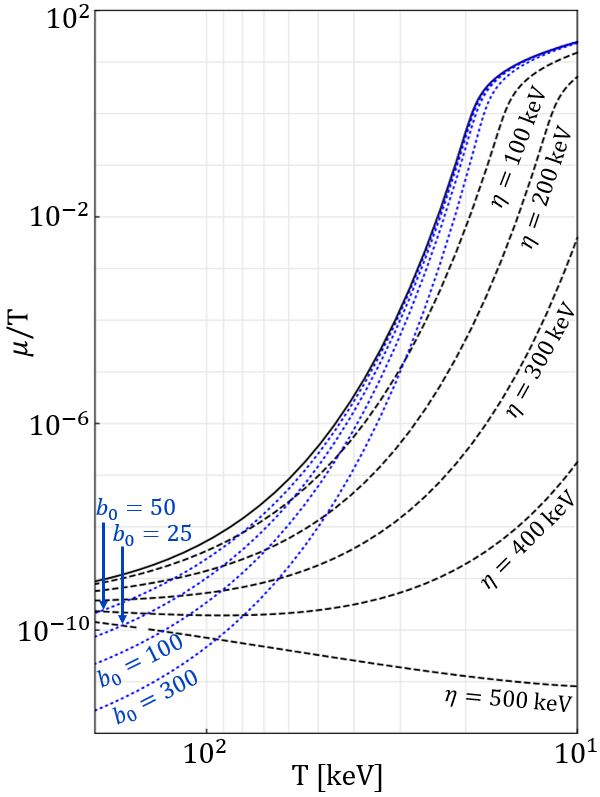
\includegraphics[width=0.5\textwidth]{plots/ChemicalPotential_04.jpg}
    \caption{The chemical potential over temperature $\mu/T$ is plotted as a function of temperature with differing values of spin potential $\eta$ (black dashed curves) and magnetic scale $b_{0}$ (blue dotted curves).}
    \label{fig:chemicalpotential}
\end{figure}
%%%%%%%%%%%%%%%%%%%%%%%%%%%%%%%%%%%%%%%

In \rf{fig:chemicalpotential} we plot the chemical potential $\mu/T$ which characterizes the importance of the charged lepton asymmetry as a function of temperature. Since the baryon (and thus charged lepton) asymmetry remains fixed, the suppression of $\mu/T$ at high temperatures indicates a large pair density which is seen explicitly in \rf{fig:densityratio}. The black line corresponds to the $b_{0}=0$ and $\eta=0$ case. The para-diamagnetic contribution from \req{paradia} does not appreciably influence $\mu/T$ until the magnetic scales involved become incredibly large well outside the observational bounds defined in \req{igmf} and \req{tbscale} as seen by the dotted blue curves of various large values $b_{0}=\{25,\ 50,\ 100,\ 300\}$. The chemical potential is also insensitive to forcing by the spin potential until $\eta$ reaches a significant fraction of the electron mass $m_{e}$ in size. The chemical potential for large values of spin potential $\eta=\{100,\ 200,\ 300,\ 400,\ 500\}\ \keV$ are also plotted as dashed black lines with $b_{0}=0$. It is interesting to note that there are crossing points where a given chemical potential can be described as either an imbalance in spin-polarization or presence of external magnetic field. While spin potential suppresses the chemical potential at low temperatures, external magnetic fields only suppress the chemical potential at high temperatures. The profound insensitivity of the chemical potential to these parameters justifies the use of the free particle chemical potential (black line) in the ranges of magnetic field strength considered for cosmology. Mathematically this can be understood as $\xi$ and $b_{0}$ act as small corrections in the denominator of \req{chem} if expanded in powers of these two parameters.

In general, an additional physical constraint is required to fully determine $\mu$ and $\eta$ simultaneously as both potentials have mutual dependency. We note that such a constraint is likely related to the total angular momentum of the considered volume. This does not necessarily imply that spin polarizations must be balanced within a single species when the orbital and spin momentum of all species in the plasma are taken into account as helicity flipping collisions between species become biased in the presence of external fields. For magnetized domains or finite volumes, boundary/surface conditions would also need to be considered.

Measurements of the CMB~\cite{aghanim2018planck} indicates that the early universe was home to domains of slightly higher and lower baryon densities which resulted in the presence of galactic super-clusters, cosmic filaments, and great voids seen today. However, the CMB, as measured today, is blind to the localized inhomogeneities required for gravity to begin galaxy and supermassive black hole formation. Such acute inhomogeneities distributed like a dust~\cite{grayson2023electronpositron} in the plasma would make the proton density spatially dependant $n_{p}\rightarrow n_{p}(x)$ which would directly affect the potentials $\mu(x)$ and $\eta(x)$ and thus the density of electrons and positrons locally. If the primordial plasma were home to such small localized magnetic domains, the associated nonzero local angular momentum within these domains would provide a natural mechanism for the formation of rotating galaxies today. Recent measurements by the James Webb Space Telescope (JWST)~\cite{yan2022first,adams2023discovery,arrabal2023spectroscopic} indicate that galaxy formation began surprisingly early at large redshift values of $z\gtrsim10$ within the first 500 million years of the universe. Additionally the observation of supermassive black holes already present~\cite{larson2023ceers} in this same high redshift period (with millions of solar masses) indicates the need for exceptionally local high density regions in the early universe whose generation is not yet explained and likely need to exist long before the recombination epoch.

% Rework the above pararaph to separate the scales of spatial anisotropies e.g. CMB is LARGE SCALE inhomogenieities while we're discussing the need for SMALL SCALE "dust" inhomogenieities which also may hide additional baryon number. Mention how LOCAL spatial effects are needed to seed early galaxies and SMBHs primordially.

%%%%%%%%%%%%%%%%%%%%%%%%%%%%%%%%%%%%%%%
\section{Electron-positron magnetization}
\label{sec:magnetization}
\noindent The magnetization of the $e^{+}e^{-}$ plasma described by the partition function in \req{boltzmann} can be written as
\begin{align}
    \label{defmagetization}
    {\cal M}\equiv\frac{T}{V}\frac{\partial}{\partial{\cal B}}\ln{{\cal Z}_{e^{+}e^{-}}} = \frac{T}{V}\left(\frac{\partial b_{0}}{\partial{\cal B}}\right)\frac{\partial}{\partial b_{0}}\ln{{\cal Z}_{e^{+}e^{-}}}\,,\qquad\frac{\partial b_{0}}{\partial{\cal B}}=\frac{e}{T^{2}}\,.
\end{align}
Magnetization arising from other components in the cosmic gas (protons, neutrinos, etc.) could in principle also be included. Localized inhomogeneities of matter evolution are often non-trivial and generally be solved numerically using magneto-hydrodynamics (MHD)~\cite{melrose2008quantum,vazza2017simulations}. In the context of MHD, primordial magnetogenesis from neutrino interactions in the electron-positron epoch was considered in~\cite{perrone2021neutrinoelectron}. We introduce dimensionless units for magnetization ${\mathfrak M}$ by defining the critical field strength
\begin{align}
    {\cal B}_{C}\equiv\frac{m_{e}^{2}}{e}\,,\qquad{\mathfrak M}\equiv\frac{\cal M}{{\cal B}_{C}}\,.
\end{align}

%%%%%%%%%%%%%%%%%%%%%%%%%%%%%%%%%%%%%%%
\begin{figure}[ht]
    \centering
    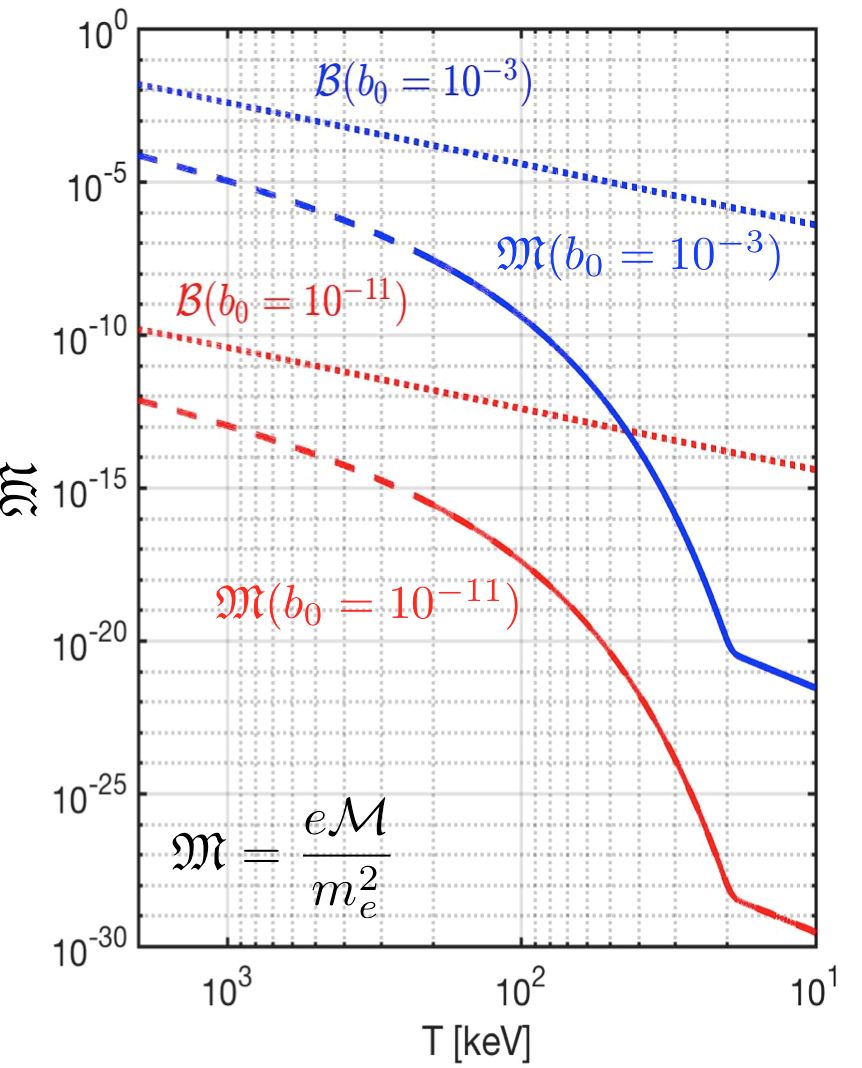
\includegraphics[width=0.5\textwidth]{Magnetization_Hc_new004.png}
    \caption{The magnetization ${\mathfrak M}$, with $g=2$, of the primordial $e^{+}e^{-}$ plasma is plotted as a function of temperature.}
    \label{fig:magnet} 
\end{figure}
%%%%%%%%%%%%%%%%%%%%%%%%%%%%%%%%%%%%%%%

The scale ${\cal B}_{C}$ is where electromagnetism is expected to become subject to non-linear effects, though luckily in our regime of interest, electrodynamics should be linear. We note however that the upper bounds of IGMFs in \req{igmf} (with $b_{0}=10^{-3}$; see \req{tbscale}) brings us to within $1\%$ of that limit for the external field strength in the temperature range considered. The total magnetization ${\cal M}$ can be broken into the sum of spin parallel ${\cal M}_{+}$ and spin anti-parallel ${\cal M}_{-}$ magnetization. We note that the expression for the magnetization simplifies significantly for $g=2$ which is the \lq\lq cusp\rq\rq\ gyro-magnetic factor~\cite{rafelski2022study} for Dirac particles. For illustration, the $g=2$ magnetization from \req{defmagetization} is then
\begin{align}
    \label{g2magplus}
    {\mathfrak M}_{+}&=\frac{e^{2}}{\pi^{2}}\frac{T^{2}}{m_{e}^{2}}\xi\cosh{\frac{\mu}{T}}\left[\frac{1}{2}x_{+}K_{1}(x_{+})+\frac{b_{0}}{6}K_{0}(x_{+})\right]\,,\qquad x_{+}=\frac{m_{e}}{T}\,,\\
    \label{g2magminus}
    -{\mathfrak M}_{-}&=\frac{e^{2}}{\pi^{2}}\frac{T^{2}}{m_{e}^{2}}\xi^{-1}\cosh{\frac{\mu}{T}}\left[\left(\frac{1}{2}+\frac{b_{0}^{2}}{12x_{-}^{2}}\right)x_{-}K_{1}(x_{-})+\frac{b_{0}}{3}K_{0}(x_{-})\right]\,,\qquad x_{-}=\sqrt{\frac{m_{e}^{2}}{T^{2}}+2b_{0}}\,.
\end{align}
As the $g$-factor of the electron is only slightly above two at $g\simeq2.00232$~\cite{tiesinga2021codata}, the above two expressions for ${\mathfrak M}_{+}$ and ${\mathfrak M}_{-}$ are only modified by a small amount because of anomalous magnetic moment (AMM). The influence of AMM would be more relevant for the magnetization of baryon gasses since the $g$-factor for protons $(g\approx5.6)$ and neutrons $(g\approx3.8)$ are substantially different from $g=2$. The influence of AMM on the magnetization of thermal systems with large baryon content (neutron stars, magnetars, hypothetical bose stars, etc.) is therefore worth exploring.

In \rf{fig:magnet}, we plot the magnetization as given by \req{g2magplus} and \req{g2magminus} with the spin potential set to unity $\xi=1$. The lower (solid red) and upper (solid blue) bounds for cosmic magnetic scale $b_{0}$ are included. The external magnetic field strength ${\cal B}/{\cal B}_{C}$ is also plotted for lower (dotted red) and upper (dotted blue) bounds. The dashed lines indicate extrapolation outside the Boltzmann limit. We place the regions outside the Boltzmann domain in dashed lines as the magnetization depends on the derivative of the partition function which may manifest differences more acutely. We see that the $e^{+}e^{-}$ plasma is overall paramagnetic and yields a positive overall magnetization which is contrary to the traditional assumption that matter-antimatter plasmas lack significant magnetic responses of their own in the bulk. With that said, the magnetization never exceeds the external field under the parameters considered which shows a lack of ferromagnetic behavior. As the universe cooled, the dropping magnetization slowed at $T_{\rm split}=20.3\keV$ where positrons vanished. Thereafter the remaining electrons density $n_{e^{-}}$ only diluted with cosmic expansion.

A curious feature of \rf{fig:magnet} is that the magnetization increases as a function of temperature. This is contrary to most systems which lose their magnetization at higher temperatures because of the disordering influence of thermal heat~\cite{huang1991statistical}. A standard feature of paramagnetic systems (Curie's law) is that the susceptibility of the material is suppressed as temperature increases, so it is natural ask: Why doesn't this occur for the primordial $e^{+}e^{-}$ plasma?

There are two reasons:
\begin{itemize}
    \item[a.] Amplification through large $n_{e^{\pm}}$ densities
    \item[b.] Conservation of magnetic flux
\end{itemize}

As discussed in \rsec{sec:abundance}, the late $e^{+}e^{-}$ plasma saw its density decrease by a factor of $10^{8}$ as the majority of the gas annihilated (seen direction in the density plotted in \rf{fig:densityratio} and indirectly through chemical potential in \rf{fig:chemicalpotential}) leaving behind only a small residual quantity of electrons. As we travel into the distance past, the overall magnetization of the plasma is supported by the density of electrons $n_{e^{-}}$ and positrons $n_{e^{+}}$ through sheer quantity.

Despite the relatively large magnetization seen in \rf{fig:magnet}, the average contribution per lepton is only a small fraction of its overall magnetic moment indicating the magnetization is only loosely organized. Specifically, the magnetization regime we are in is described by
\begin{align}
    \label{fractionalmagnetization}
    {\cal M}V\ll\mu_{B}(N_{e^{+}}+N_{e^{-}})\,,\qquad\mu_{B}=\frac{e}{2m}\,,
\end{align}
where $\mu_{B}$ is the Bohr magneton and $N=nV$ is the total particle number in the proper volume. To better demonstrate that the plasma is only weakly magnetized, we define the average magnetic moment per lepton given by along the field ($z$-direction) axis as
\begin{align}
    \label{momentperlepton}
    \vert\vec{m}\vert_{z}\equiv\frac{{\cal M}}{n_{e^{-}}+n_{e^{+}}}\,,\qquad\vert\vec{m}\vert_{x}=\vert\vec{m}\vert_{y}=0\,.
\end{align}
From spin statistics, we expect the transverse expectation values to be zero. The quantity defined in \req{momentperlepton} gives us an insight into the microscopic response of the plasma.

The average magnetic moment $\vert\vec{m}\vert_{z}$ defined in \req{momentperlepton} is plotted in \rf{fig:momentperlepton} which displays how essential the external field is on the \lq per lepton\rq\ magnetization. Both the $b_{0}=10^{-11}$ (lower plot, red curve) and $b_{0}=10^{-3}$ (upper plot, blue curve) cosmic magnetic scale bounds are plotted in the Boltzmann approximation. The dashed lines indicate where this approximation is only qualitatively correct. For illustration, a constant magnetic field case (solid green line) with a comoving reference value chosen at temperature $T_{0}=10\keV$ is also plotted. If the field strength is held constant, then the average magnetic moment per lepton is suppressed at higher temperatures as expected for magnetization satisfying Curie's law. The difference between the non-constant (red and blue solid curves) case and the constant field (solid green curve) case demonstrates the importance of the conservation of primordial magnetic flux in the plasma, required by \req{bscale}. The conservation of flux through comoving surfaces for the external field ensures that as we travel into the past, the increasing magnetic field enhances the overall magnetization of the gas. While not shown, if \rf{fig:momentperlepton} was extended to lower temperatures, the magnetization per lepton of the constant field case would be greater than the non-constant case which agrees with our intuition that magnetization is easier to achieve at lower temperatures.

%%%%%%%%%%%%%%%%%%%%%%%%%%%%%%%%%%%%%%%
\begin{figure}[ht]
    \centering
    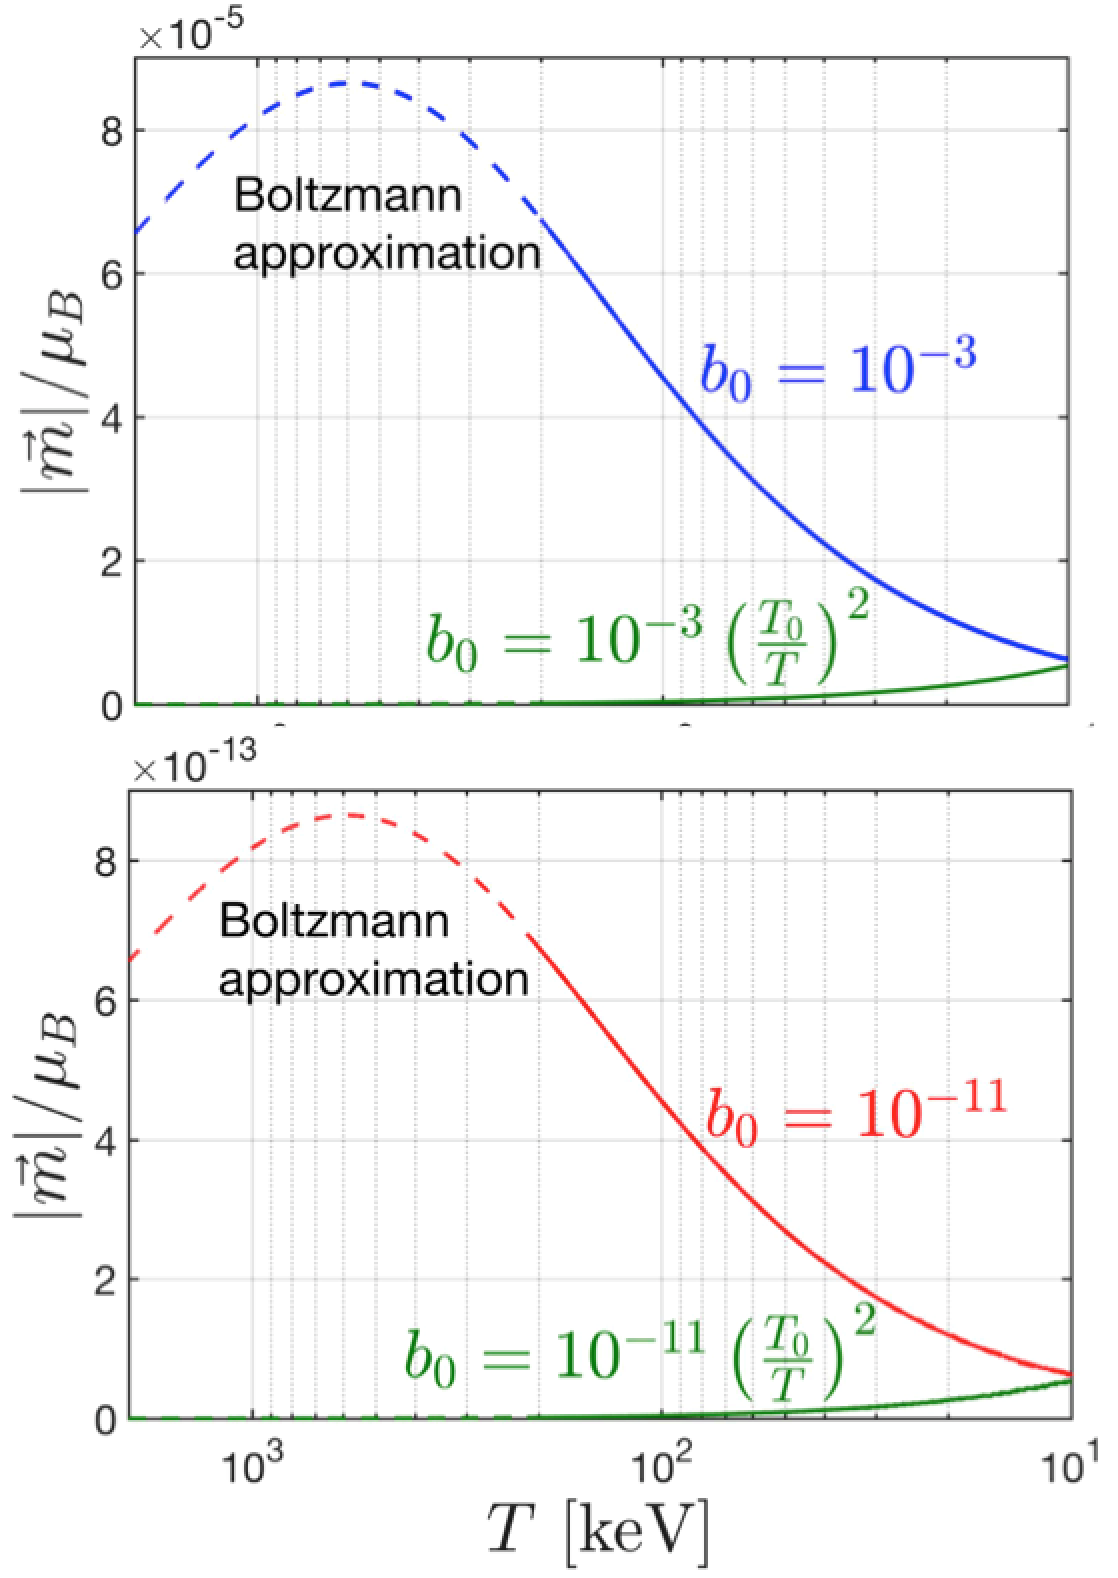
\includegraphics[width=0.5\textwidth]{plots/NewMagnetizationDensity004_Boltz.png}
    \caption{The magnetic moment per lepton $\vert\vec{m}\vert_{z}$ along the field axis.}
    \label{fig:momentperlepton}
\end{figure}
%%%%%%%%%%%%%%%%%%%%%%%%%%%%%%%%%%%%%%%

%%%%%%%%%%%%%%%%%%%%%%%%%%%%%%%%%%%%%%%
\section{Spin potential and ferromagnetism}
\label{sec:spin}
\noindent Up to this point, we have neglected the impact that a nonzero spin potential $\eta\neq0$ (and thus $\xi\neq1$) would have on the primordial $e^{+}e^{-}$ plasma magnetization. In the limit that the cosmic magnetic scale $b_{0}$ (and thus external magnetic field) goes to zero, the magnetization given in \req{g2magplus} and \req{g2magminus} is entirely controlled by the spin fugacity $\xi$ asymmetry generated by the spin potential $\eta$ yielding
\begin{align}
    \label{ferro}
    \lim_{b_{0}\rightarrow0}{\mathfrak M}=\frac{e^{2}}{\pi^{2}}\frac{T^{2}}{m_{e}^{2}}\sinh{\frac{\eta}{T}}\cosh{\frac{\mu}{T}}\left[\frac{m_{e}}{T}K_{1}\left(\frac{m_{e}}{T}\right)\right]+{\cal O}(b_{0})\,,\\
    \label{asymmetry}
    2\sinh{\frac{\eta}{T}}=\xi-\xi^{-1}\,.
\end{align}
Given \req{ferro}, we can understand the spin potential as a kind of ferromagnetic influence on the primordial gas which allows for magnetization even in the absence of external magnetic fields. As $\sinh{\eta/T}$ is an odd function, the sign of $\eta$ also controls the alignment of the magnetization. In general, $\eta=\eta(\mu,T)$ is a function of the chemical potential and temperature. As discussed in \rsec{sec:fugacity}, the two potentials are mutually related and likely would need be simultaneously solved.

One exploratory model is to describe the required spin polarization asymmetry, described in \req{spotential}, to generate a homogeneous magnetic field which dissipates as the universe cools down. In this model, there is no external primordial magnetic field generated by some unrelated physics, but rather the $e^{+}e^{-}$ plasma itself is responsible for the field by virtue of spin polarization. This would obey the following assumption of
\begin{align}
    \label{selfmag}
    {\mathfrak M}\leftrightarrow\frac{\cal B}{{\cal B}_{C}}=\frac{b_{0}T^{2}}{e{\cal B}_{C}}\,.
\end{align}

The result of the self-magnetization assumption in \req{selfmag} is plotted in \rf{fig:self}. The solid lines indicate the curves for $\eta/T$ which become dashed above $T=300\keV$ to indicate that the Boltzmann approximation is no longer appropriate. The dashed lines are the curves for the chemical potential $\mu/T$. We note that unlike the chemical potential which is insensitive to $\eta$ until it reaches larger values, the magnetization is strongly dependant on any external forcing of spin polarization asymmetry. What is of more interest is the natural scale of the magnetization that even a small spin fugacity ($\eta<1\eV$) fits easily within the bounds of the predicted magnetization during this era if the IGMF measured today was of primordial origin. The reason for this is that the magnetization seen in \req{g2magplus} - \req{g2magminus} and \req{ferro} are scaled by $\alpha{\cal B}_{C}$ where $\alpha\propto e^{2}$ is the fine structure constant.

%%%%%%%%%%%%%%%%%%%%%%%%%%%%%%%%%%%%%%%
\begin{figure}[ht]
    \centering
    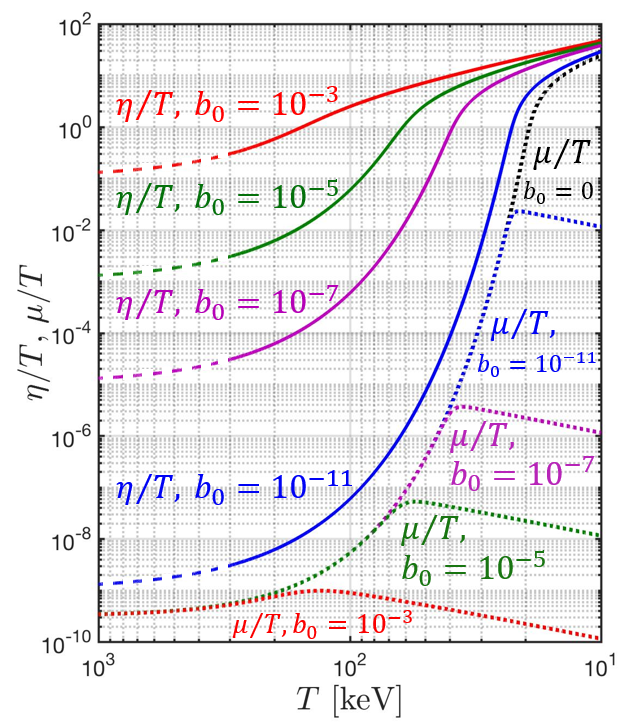
\includegraphics[width=0.5\textwidth]{plots/Spinchemical_02.png}
    \caption{The spin potential $\eta$ (solid lines) and chemical potential $\mu$ (dotted lines) are plotted under the assumption of self-magnetization through a nonzero spin polarization in bulk of the plasma.}
    \label{fig:self} 
\end{figure}
%%%%%%%%%%%%%%%%%%%%%%%%%%%%%%%%%%%%%%%

%%%%%%%%%%%%%%%%%%%%%%%%%%%%%%%%%%%%%%%
%\begin{figure}[ht]
%    \centering
%    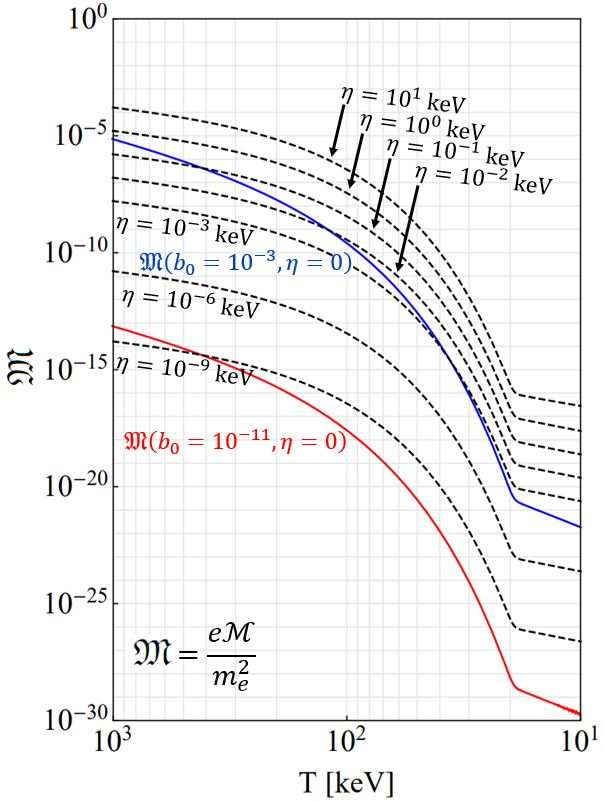
\includegraphics[width=0.5\textwidth]{plots/SpinPolarizationEffect_04.jpg}
%    \caption{The magnetization ${\mathfrak M}$ for various values of $\eta$ (dashed black lines) with zero external field are compared to the magnetization with external fields (blue and red) with $\eta=0$.}
%    \label{fig:ferro} 
%\end{figure}
%%%%%%%%%%%%%%%%%%%%%%%%%%%%%%%%%%%%%%%

%%%%%%%%%%%%%%%%%%%%%%%%%%%%%%%%%%%%%%%
\begin{figure}[ht]
    \centering
    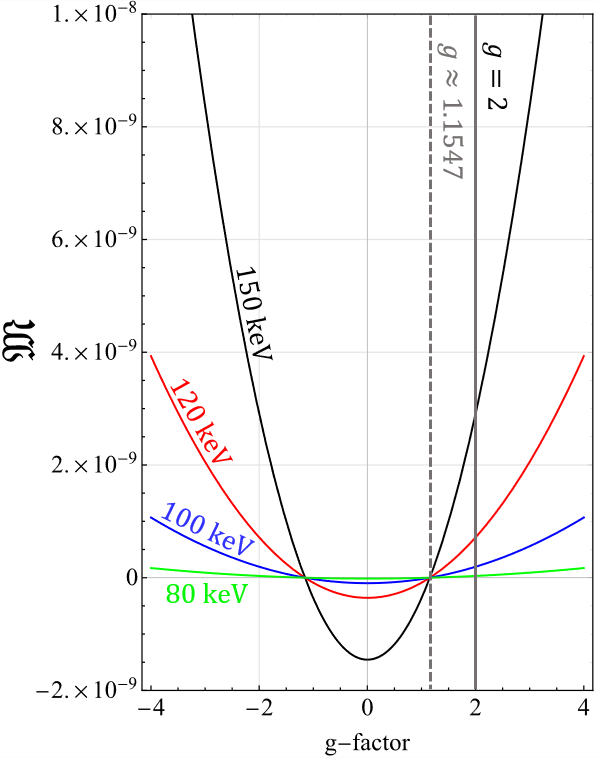
\includegraphics[width=0.5\textwidth]{plots/GFactor_02.png}
    \caption{TBW.}
    \label{fig:gfac} 
\end{figure}
%%%%%%%%%%%%%%%%%%%%%%%%%%%%%%%%%%%%%%%

%%%%%%%%%%%%%%%%%%%%%%%%%%%%%%%%%%%%%%%
\section{Closing}
\label{sec:conclusions}
\noindent In this work, we explored the primarily paramagnetic magnetization of the $e^{+}e^{-}$ thermal Fermi gas in the temperature range of the early universe between $2,000\keV>T>20\keV$. The combination of strong magnetic fields, high matter-antimatter density, and relatively high temperatures (far higher than the Sun's core temperature~\cite{bahcall2001solar} of $T_{\odot}=1.37\keV$) make this universe era unique in cosmology and astrophysics.

We show that the primordial universe $e^{+}e^{-}$ plasma has paramagnetic properties when subjected to an external field. This response surprisingly does not diminish in the distant past with high temperature unlike most magnetic phenomenon, but is enhanced due to
\begin{itemize}
    \item[a] the high density of electron-positron pairs which exist in the plasma during this era and
    \item[b] the conservation of magnetic flux in an expanding universe which helps maintain the polarization of the plasma.
\end{itemize}

Future opportunities include studying further the influence of spin polarization imbalances (say in the photon, or neutrino sectors) which may manifest as self-magnetization or ferromagnetic-like phenomenon in the primordial universe. An additional avenue of research is studying spatial homogeneities. As the chemical potential of $e^{+}e^{-}$ is sensitive to the baryon density, any local spatial variations can effect magnetization substantially. Recent measurements by the JWST indicate that large-scale structure, galactic, and supermassive black hole formation occurred earlier than expected which may indicate unusual matter agglomeration in even primordial eras.

%%%%%%%%%%%%%%%%%%%%%%%%%%%%%%%%%%%%%%%
\bibliographystyle{unsrtnat}
\bibliography{refs-plasma-partition}
%%%%%%%%%%%%%%%%%%%%%%%%%%%%%%%%%%%%%%%

\end{document}
